\documentclass[11pt]{article}

\usepackage{graphicx}
\usepackage{amsmath}
\usepackage{fancyvrb}

\title{An ARIMA Analysis on VIX}
\author{Gerardo Dur\'an Mart\'in}

\begin{document}
\maketitle
\section{VIX}
According to the Chicago Board Option Exchange (CBOE),
\begin{quotation}
	`` The CBOE Volatility Index (VIX Index) is a key measure of market expectations of near-term volatility conveyed by S\&P 500 stock index option prices. Since its introduction in 1993, the VIX Index has been considered by many to be the world's premier barometer of investor sentiment and market volatility[].��
\end{quotation}

\begin{figure*}[h]
	\centering
	\includegraphics[scale=0.4]{../images/VIX.pdf}
	\caption{VIX Sample Dataset}
\end{figure*}

The goal of this narrow essay is to show the basic ideas about how one goes about choosing the parameters for fitting an ARIMA model. This is not intended to be a comprehensive writing about ARIMA, so much as it is about how to apply on a first instance these kinds of models.\\

Herein we will present an example of fitting an ARIMA model to the VIX index, from the point of view of a trader interested in predicting volatility. Understanding volatility allows one to understand more about the risk associated in some trades and the market conditions at a given point in time. To understand how volatile one market is, one can quantify the potential losses to occur.

\section{Predicting the VIX}
The sample of the VIX we will be working on goes from the first of April, 2010, and ends at the eighteen of may, 2017.\\

Before fitting an ARIMA model, the first step is to test whether the sample we have contains within a predictive pattern to extract from a model. To do so, we chose the Phillip-Perron test of unit root. Recall that the assumptions from this model are:
\begin{align*}
	H_0: \exists \text{ unit root}\\
	H_a: \not\exists\text{ unit root}
\end{align*}

Using the \texttt{Statsmodels} python package we see the following\\

\begin{figure*}[h]
\centering
\begin{BVerbatim}[fontsize=\tiny]
	     Phillips-Perron Test (Z-tau)    
	=====================================
	Test Statistic                 -5.826
	P-value                         0.000
	Lags                                1
	-------------------------------------

	Trend: Constant
	Critical Values: -3.43 (1%), -2.86 (5%), -2.57 (10%)
	Null Hypothesis: The process contains a unit root.
Alternative Hypothesis: The process is weakly stationary.\end{BVerbatim}
\end{figure*}

Which asserts proposed hypothesis: the null hypothesis can be rejected, the model does not contain a unit root, ergo, there exists a pattern in the data.\\

We now start choosing the parameters of the ARIMA model to fit. First, we desire to know whether this process is integrated and, if so, which order. This can be visualized by plotting the first difference of the VIX.\\

\begin{figure*}[h]
	\centering
	\includegraphics[scale=0.4]{../images/VIX_diff}
	\caption{VIX differences}
	\label{fig:vix_diff}
\end{figure*}

Figure \ref{fig:vix_diff}, along with the Phillip-Perron test indicate a possible integrated model with order 1 or 0.\\

To continue this analysis we set out to plot the partial correlation function and the correlation function in order to visually get an idea of the $p$ and $q$ parameters of the model we desire to fit.\\

\begin{figure*}[h]
	\centering
	\includegraphics[scale=0.4]{../images/pacf}
	\caption{Partial Autocorrelation Function}
	\label{fig:pac}
\end{figure*}

\begin{figure*}[h]
	\centering
	\includegraphics[scale=0.4]{../images/acf}
	\caption{Autocorrelation Function}
	\label{fig:ac}
\end{figure*}

Looking at figures \ref{fig:pac} and \ref{fig:ac} we can start trying to fit our ARIMA model by way of trial and error. In this case, a AR(1) I(0) MA(0) was the model whose parameters best suited our model.

\newpage

We can explain the latter result as follows: due the behavior of the VIX, we cannot express the process to take a random walk, that is the reason of I(0). Furthermore, the process does seem to have an autoregressive factor, and that is why we chose to fit AR(1). Finally, since the model does not seem to have a moving average component, we fit a MA(0), which gave significant coefficients in the model.\\

\begin{figure*}[h]
\centering
\begin{BVerbatim}[fontsize=\tiny]
                          Results: ARMA
====================================================================
Model:              ARMA             BIC:                 7071.1949 
Dependent Variable: VIX              Log-Likelihood:      -3524.3   
Date:               2017-05-21 13:55 Scale:               1.0000    
No. Observations:   1857             Method:              css-mle   
Df Model:           2                Sample:              01-04-2010
Df Residuals:       1855                                  05-18-2017
Converged:          1.0000           S.D. of innovations: 1.613     
AIC:                7054.6148        HQIC:                7060.726  
----------------------------------------------------------------------
             Coef.    Std.Err.      t       P>|t|     [0.025    0.975]
----------------------------------------------------------------------
const       17.6069     0.9448    18.6346   0.0000   15.7550   19.4587
ar.L1.VIX    0.9609     0.0064   151.2733   0.0000    0.9484    0.9733
-----------------------------------------------------------------------------
                 Real           Imaginary          Modulus          Frequency
-----------------------------------------------------------------------------
AR.1            1.0407             0.0000           1.0407             0.0000
====================================================================
\end{BVerbatim}
\end{figure*}

The Jarque-Bera test was used to asses normality. The test were conclusive, the residuals did not appear to distribute normally. The distribution of the residuals seemed to be platykurtic thus breaking the assumption of normality in the data.

\newpage

\begin{figure*}[h]
	\centering
	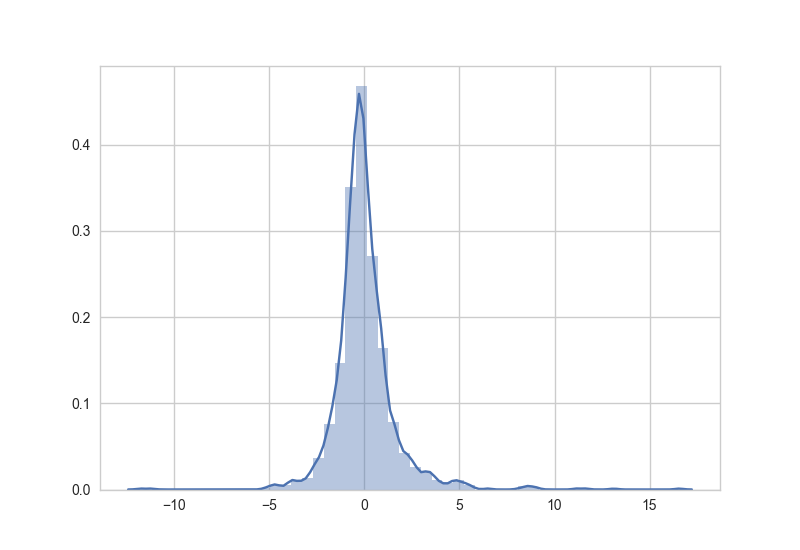
\includegraphics[scale=0.4]{../images/resid_dist}
	\caption{Distribution of Residuals}
\end{figure*}


Nonetheless, to have residuals with thinner tails than a normal distribution is positive for the purposes of the model since this implies less uncertainty about the model we are fitting. A better way to approximate model could be to model the residuals with a distribution such that has less variance than a normal distribution.
\end{document}